Para el desarrollo de esta práctica se utilizó el lenguaje de programación Python en su versión 3.10, con el que se diseñó un conjunto de scripts y una libreta de Jupyer para cumplir con los objetivos de la práctica.

\subsection{Conjunto de datos utilizado}
El conjunto de datos utilizado para esta práctica consta de una colección cuyo objetivo es la predicción de un derrame cerebral (stroke, en inglés). Dicho conjunto de datos fue obtenido de la plataforma Kaggle, y consta de 10 atributos de diversos tipos y 1 variable objetivo, teniendo un total de 40,910 instancias. El conjunto de datos contiene 2 clases en la variable objetivo, las cuales se encuentran balanceadas en porciones del 50\%. Los tipos de datos disponibles en el conjunto de datos empleado son:

\begin{itemize}
	\item Ordinales
	\begin{itemize}
		\item age	
	\end{itemize}
	
	\item Continuos
	\begin{itemize}
		\item avg\_glucose\_level
		\item bmi
	\end{itemize}
	
	\item Categóricos
	\begin{itemize}
		\item sex
		\item hypertension
		\item heart\_disease
		\item ever\_married
		\item work\_type
		\item residence\_type
		\item smoking\_status
		\item stroke (variable objetivo)
	\end{itemize}
\end{itemize}

\subsection{Pre-procesamiento de datos}
\subsubsection{Imputación de datos}
El conjunto de datos contaba con 3 instancias con datos faltantes en el atributo \emph{sex}. Dada la gran cantidad de instancias disponibles, se optó por rellenar estos valores faltantes usando el valor más frecuente de dicho atributo. En la Figura \ref{Fig: Imputation} se puede observar la distribución del atributo \emph{sex} posterior al proceso de imputación.

\begin{figure}[htbp]
	\centering
	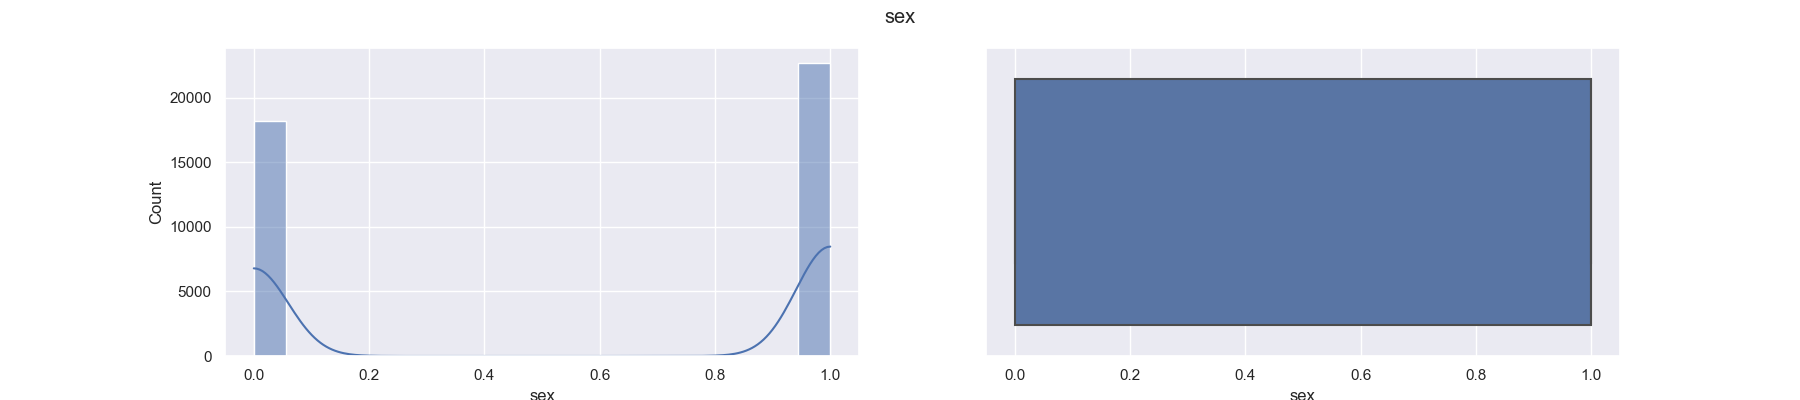
\includegraphics[width=\textwidth]{sex_distribution}
	\caption{Distribución de los datos posterior a la imputación aplicada al atributo \emph{sex}.}
	\label{Fig: Imputation}
\end{figure}

\subsubsection{Normalización de datos}
Se realizó un proceso de obtención de la distribución de los datos que conforman el conjunto de datos, usando histogramas y diagramas de cajas. Se pudo observar que para los atributos continuos se contaba con una distribución de tipo uniforme, por lo que se usó el método z-score para normalizar los datos. Para el resto de atributos, dada su naturaleza categórica y ordinal, se optó por no realizar algún tipo de normalización.

Las Figuras \ref{Fig: glucose_norm} y \ref{Fig: bmi_norm} muestran la una comparación entre la distribución de los atributos previa y posterior a normalizar.

\begin{figure}[!htb]
	\centering
	\begin{subfigure}[b]{0.85\textwidth}
		\centering
		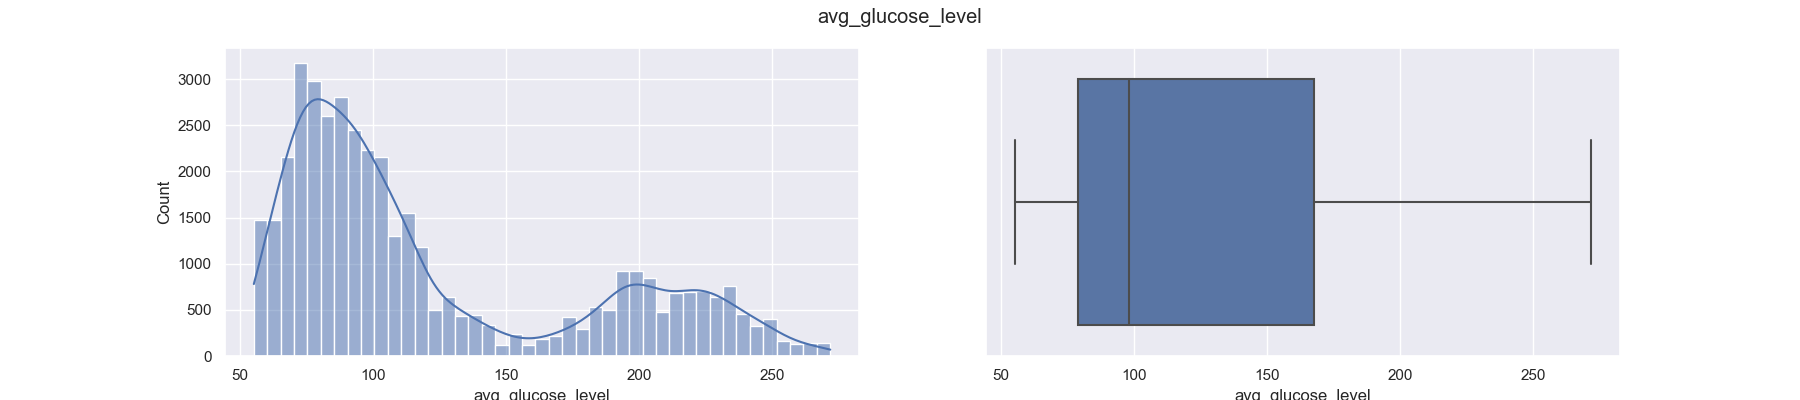
\includegraphics[width=\textwidth]{avg_glucose_level_distribution}
		\caption{Histograma de atributo \emph{avg\_glucose\_level} sin normalizar.}
	\end{subfigure}
	\hfill
	\begin{subfigure}[b]{0.85\textwidth}
		\centering
		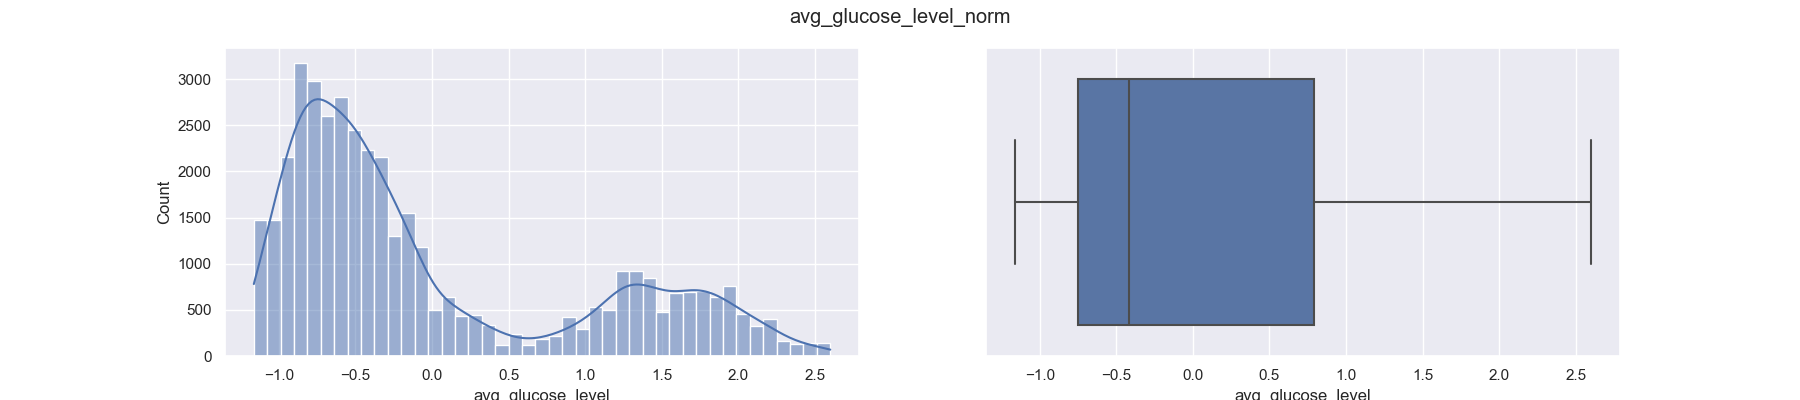
\includegraphics[width=\textwidth]{avg_glucose_level_distribution_norm}
		\caption{Histograma de atributo \emph{avg\_glucose\_level} posterior a normalización.}
	\end{subfigure}
	\caption{Normalización de atributo \emph{avg\_glucose\_level}.}
	\label{Fig: glucose_norm}
\end{figure}

\begin{figure}[!htb]
	\centering
	\begin{subfigure}[b]{0.85\textwidth}
		\centering
		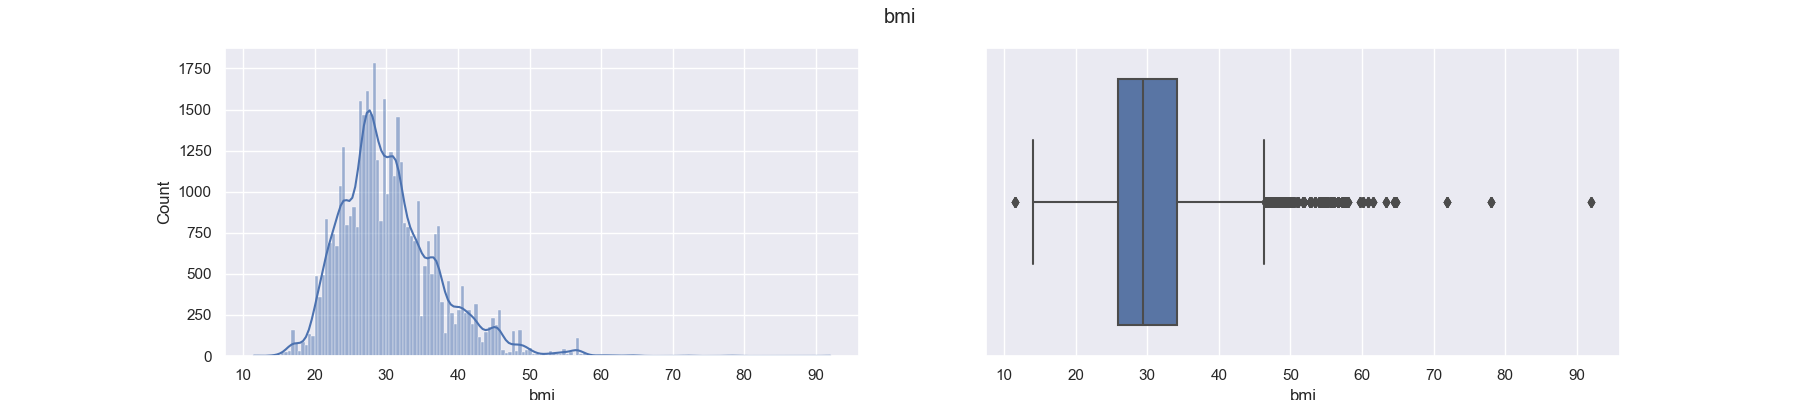
\includegraphics[width=\textwidth]{bmi_distribution}
		\caption{Histograma de atributo \emph{bmi} sin normalizar.}
	\end{subfigure}
	\hfill
	\begin{subfigure}[b]{0.85\textwidth}
		\centering
		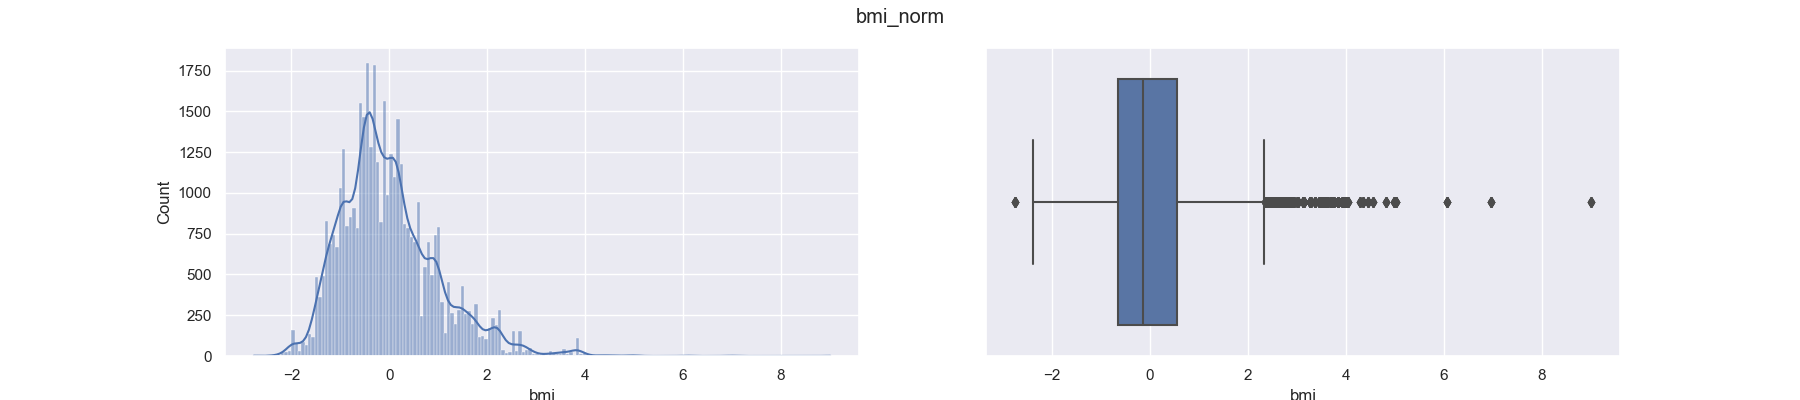
\includegraphics[width=\textwidth]{bmi_distribution_norm}
		\caption{Histograma de atributo \emph{bmi} posterior a normalización.}
	\end{subfigure}
	\caption{Normalización de atributo \emph{bmi}.}
	\label{Fig: bmi_norm}
\end{figure}

\FloatBarrier
\subsection{Selección de atributos}
Con el fin de obtener una perspectiva general del desempeño del algoritmo KNN al usar diferentes tipos de datos, se optó por utilizar 3 métodos distintos para extracción de atributos.

\subsubsection{Método Pearson}
Utilizando la matriz de correlación de Pearson, se generó un mapa de calor para determinar los atributos más correlacionados con la variable objetivo. De este análisis se tomaron los 3 atributos con mayor índice de correlación.

En la Figura \ref{Fig: Pearson} se puede observar el mapa de calor obtenido tras en análisis de correlación de Pearson. Donde se puede concluir que los atributos con mayor correlación con la variable objetivo (\emph{stroke}) son: \emph{avg\_glucose\_level}, \emph{hypertension} y \emph{heart\_disease}

\begin{figure}[htbp]
	\centering
	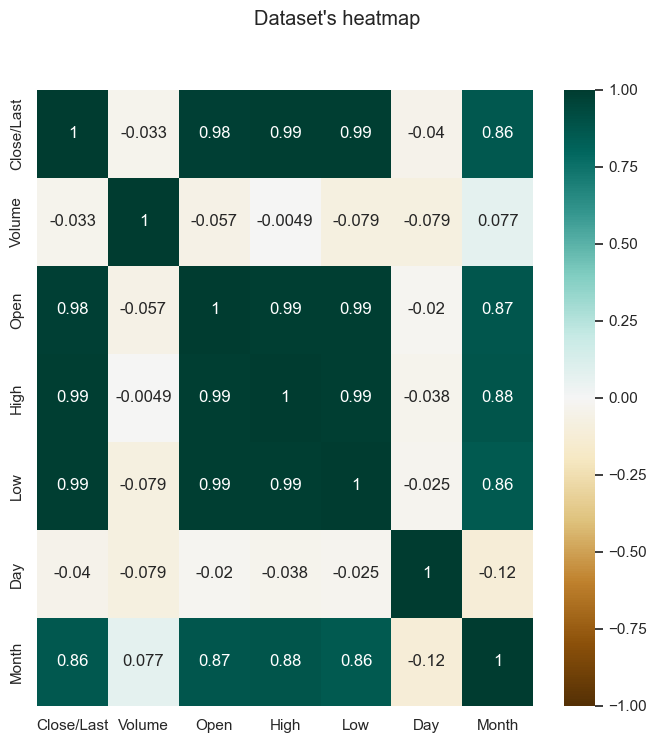
\includegraphics[width=0.8\textwidth]{dataset_heatmap}
	\caption{Mapa de calor obtenido tras el análisis de correlación de Pearson.}
	\label{Fig: Pearson}
\end{figure}

\subsubsection{Método PCA}
Utilizando el método de PCA para generar un subespacio que comprima la información global del conjunto de datos, se obtuvieron 3 componentes principales del conjunto de datos.

En la Tabla \ref{Tab: PCA} se observa una muestra de 10 elementos de los 3 componentes principales resultantes del método PCA.

\begin{table}[htbp]
	\centering
	\caption{Muestra de los 3 componentes principales generados por PCA.}
	\begin{tabular}{ccc}
		\hline\hline
		PC1    & PC2   & PC3    \\ 
		\hline\hline
		-62.99 & 2.71  & 1.65   \\
		-41.99 & 8.22  & 2.87   \\
		-61.00 & 0.33  & 0.57   \\
		-40.99 & 0.64  & 0.80   \\
		-84.99 & 1.01  & -0.03  \\
		-54.99 & -0.46 & 1.00   \\
		-82.00 & -0.82 & 0.43   \\
		-16.99 & -0.12 & 1.12   \\
		-30.99 & 0.91  & 1.00   \\
		-55.00 & -0.11 & 0.71   \\
		\hline\hline
	\end{tabular}
	\label{Tab: PCA}
\end{table}

\subsubsection{Selección experimental}
Mediante el apoyo de una pairplot de la biblioteca \emph{Seaborn}, se busca a los atributos que mejor logren separar visualmente a la variable objetivo. Dichos atributos se seleccionan para realizar el entrenamiento del modelo.

Para el caso de nuestro conjunto de datos, la Figura \ref{Fig: Experimental} muestra el pairplot resultante, donde se puede observar que los atributos que proporcionan una mejor separación de la variable objetivo son \emph{age}, \emph{avg\_glucose\_level} y \emph{bmi}.

\begin{figure}[htbp]
	\centering
	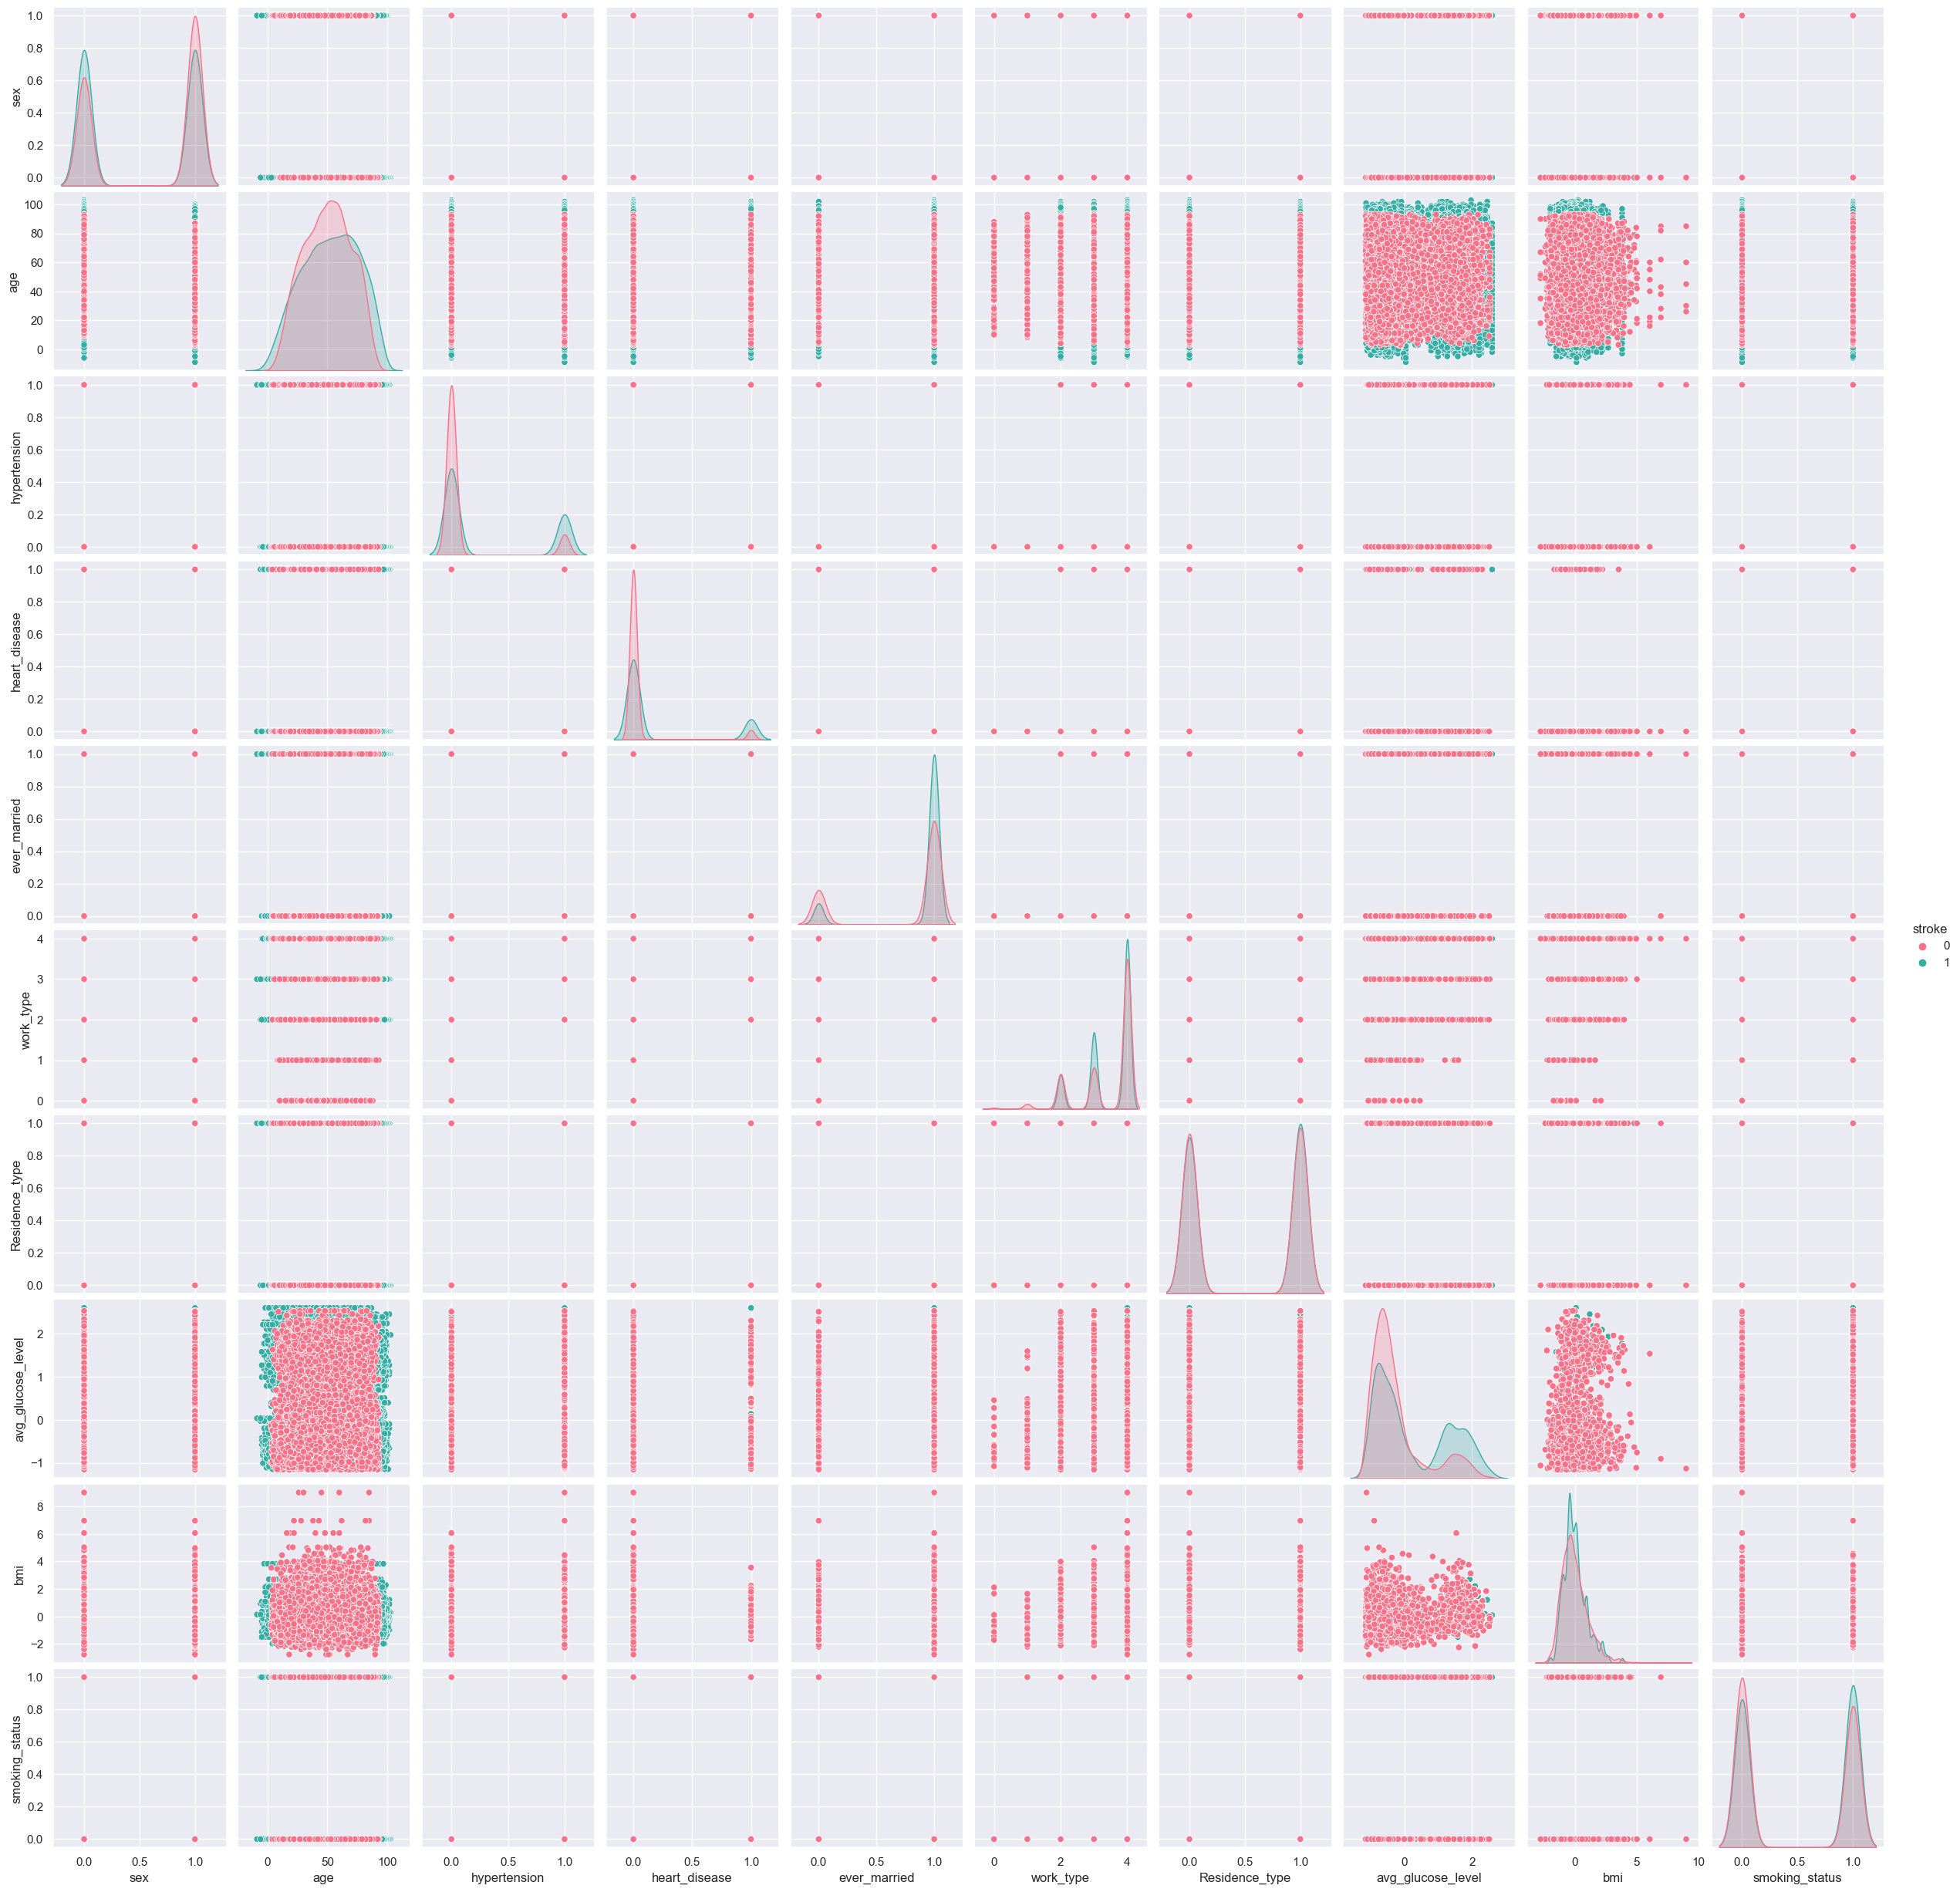
\includegraphics[width=\textwidth]{dataset_pairplot}
	\caption{Pairplot obtenido del conjunto de datos.}
	\label{Fig: Experimental}
\end{figure}

\FloatBarrier
\subsection{Implementación de KNN}
El Algoritmo \ref{Alg: KNN} muestra el pseudocódigo utilizado para implementar el algoritmo KNN dentro del contexto de la práctica.

\begin{algorithm}
\caption{Clasificador KNN}
\begin{algorithmic}[1]
\Procedure{KNN}{$X_{\text{train}}, y_{\text{train}}, X_{\text{test}}, k$}
    \For{$\text{instancia} \in X_{\text{test}}$}
        \State Calcular la distancia entre la instancia actual y todas las instancias en $X_{\text{train}}$
        \State Ordenar las distancias de menor a mayor
        \State Tomar los $k$ vecinos más cercanos
        \State Obtener las etiquetas correspondientes a los $k$ vecinos más cercanos
        \State Realizar la votación mayoritaria para determinar la etiqueta predicha
        \State Asignar la etiqueta predicha a la instancia actual
    \EndFor
    \State Retornar las etiquetas predichas para todas las instancias en $X_{\text{test}}$
\EndProcedure
\end{algorithmic}
\label{Alg: KNN}
\end{algorithm}

\subsection{Evaluación de algoritmo}
Se realizó un proceso de evaluación para cada uno de los conjuntos de datos generados por las técnicas de selección de características. Estas evaluaciones consistieron en la obtención de la matriz de confusión y las métricas exactitud, sensibilidad, precisión y puntaje F1. Dicho proceso de evaluación se realizó sobre el 30\% del conjunto de datos.
